\chapter{Diagramme de classes}

\section{Diagramme}

\begin{figure}
  \centering
  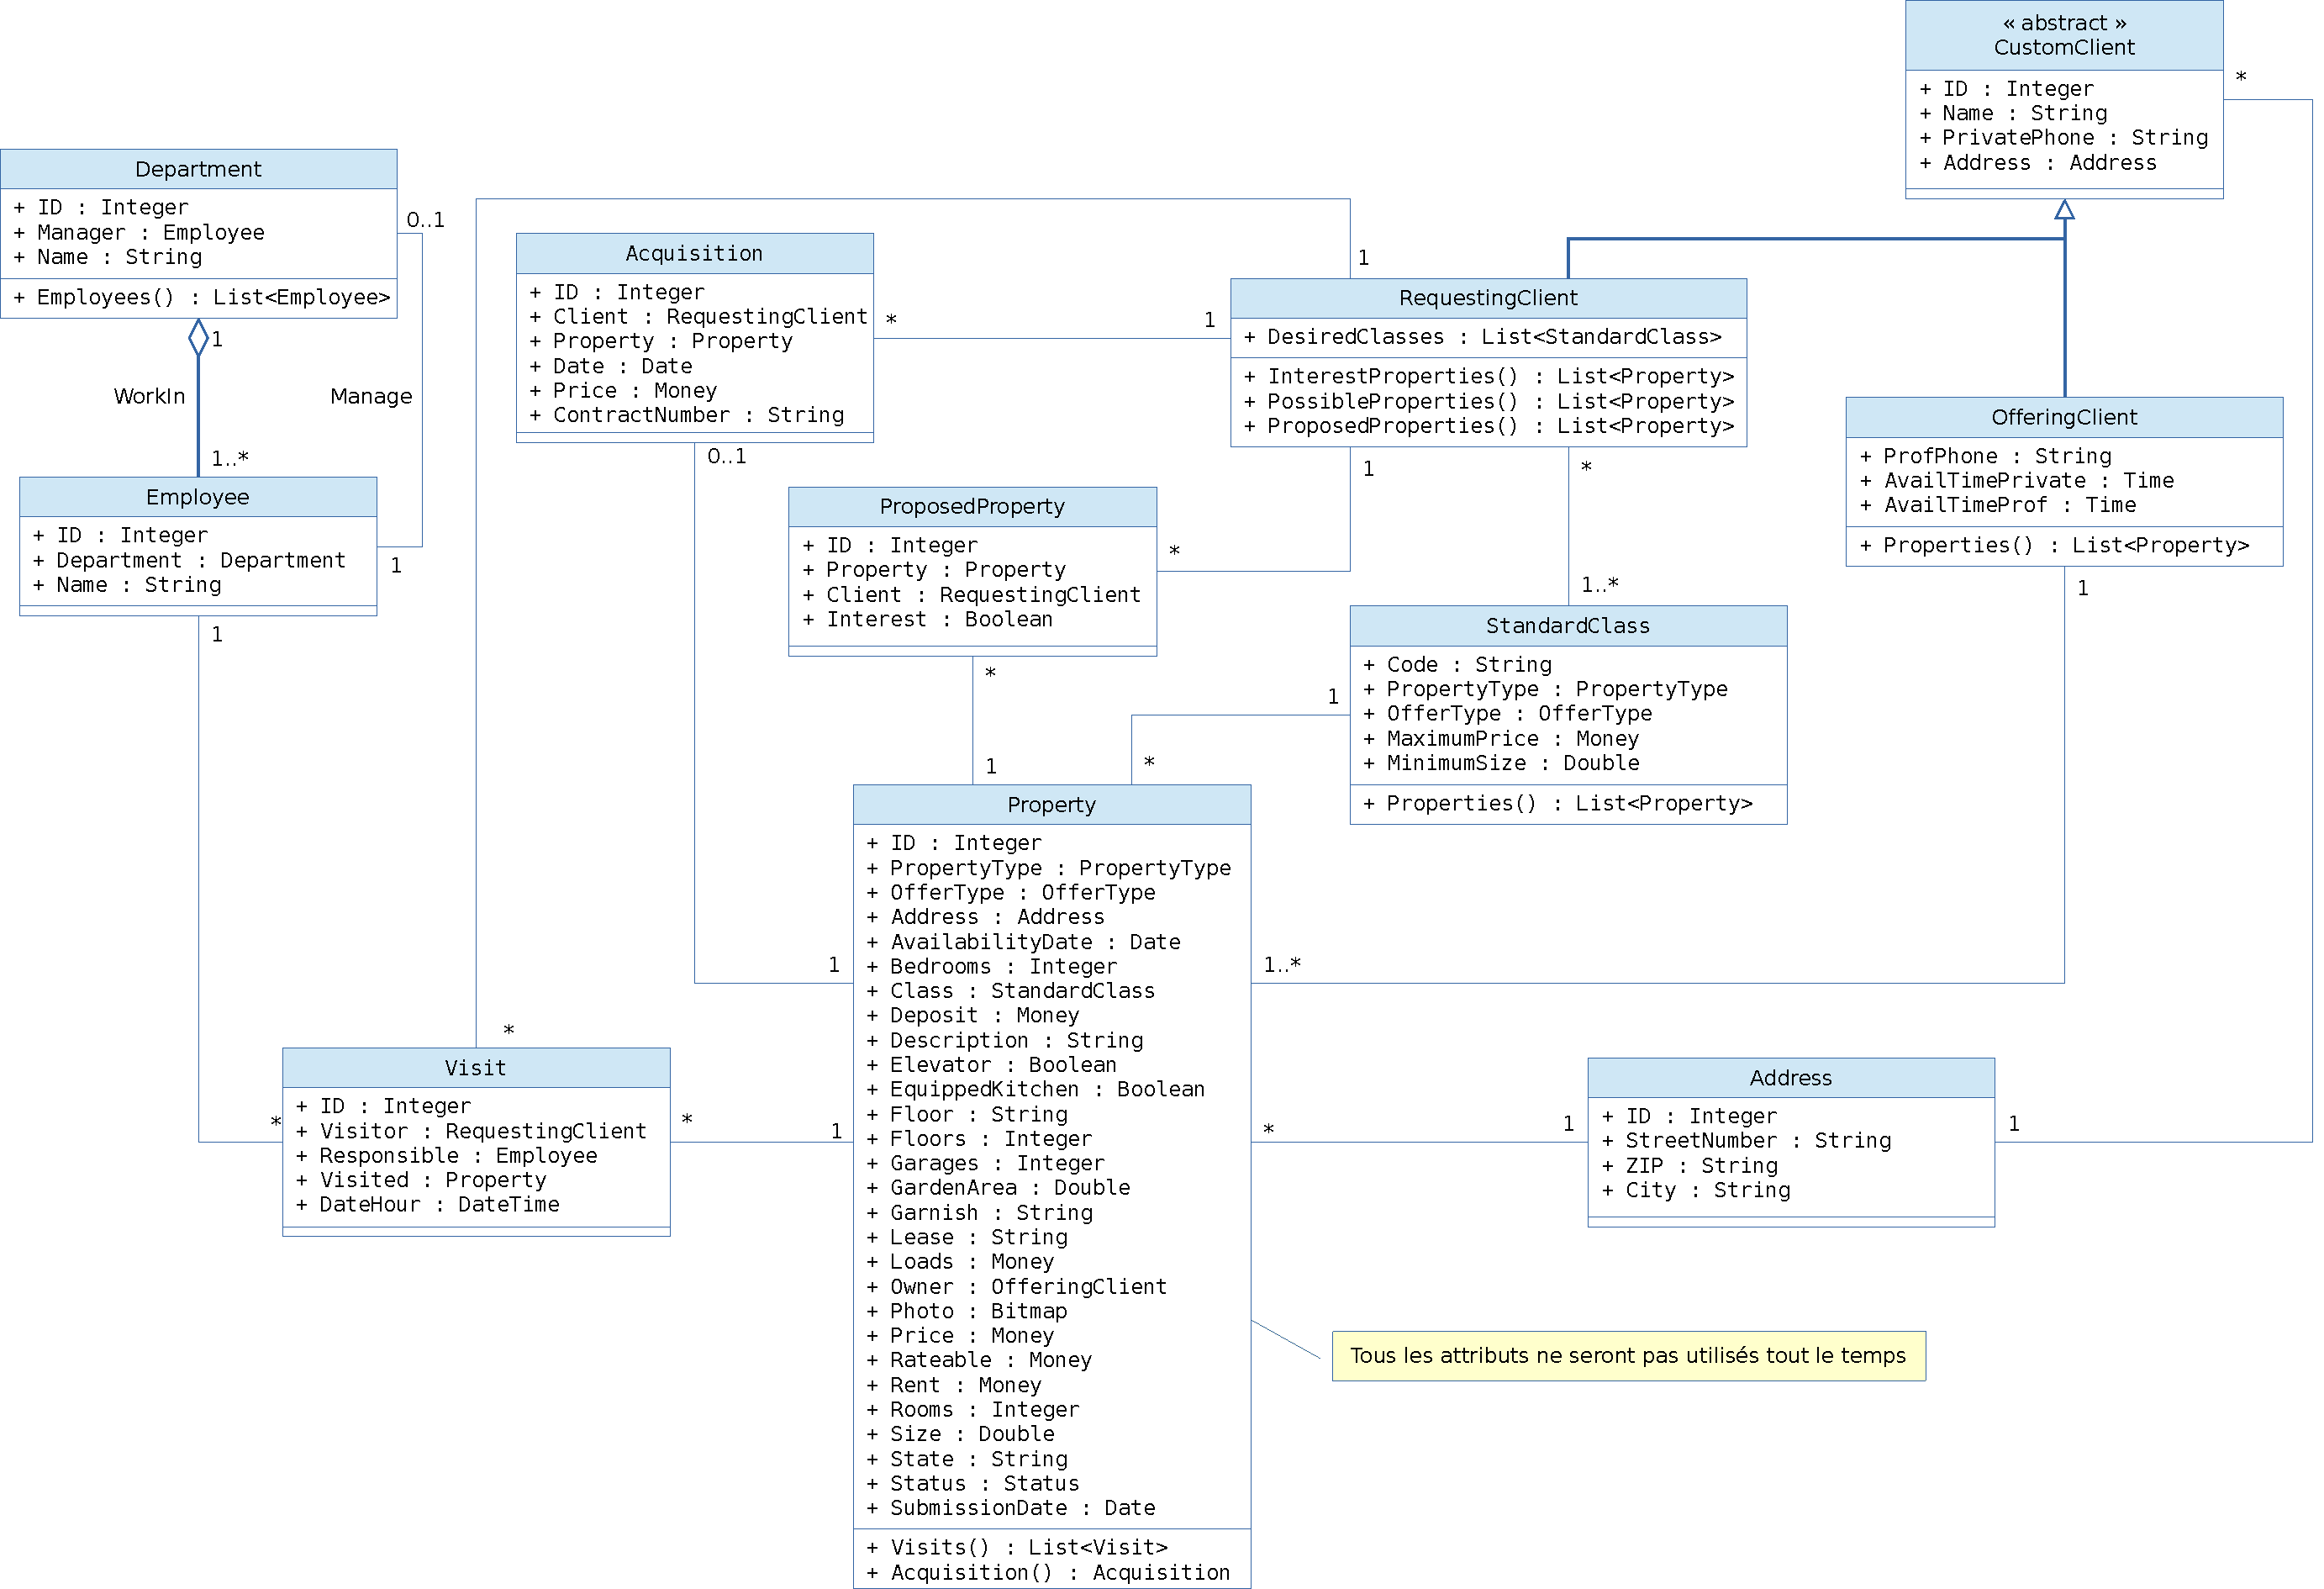
\includegraphics[angle=90,height=0.99\textheight]{IMG/cd}
  \caption{Diagramme de classes}
  \label{img_cd}
\end{figure}

La figure \refpage{img_cd} illustre le diagramme de classes du projet.

\section{Documentation technique}

La description des classes est reprise dans la table \refpage{tbl_description_classes}. Les contraintes de ce diagramme figurent dans le tableau \refpage{tbl_business_rules}.

Le type \code{PropertyType} est une énumération des éléments suivants: \og{}studio\fg{}, \og{}appartement\fg{}, \og{}maison\fg{}, \og{}entrepôt\fg{}, \og{}emplacement\fg{} et \og{}terrain\fg{}. Le type \code{OfferType} est une énumération des éléments suivants: \og{}location\fg{}, \og{}vente\fg{}. Le type \code{Status} est une énumération des éléments suivants: \og{}disponible\fg{}, \og{}loué\fg{}, \og{}acheté\fg{}. Ces énumérations pourront évoluer si nécessaire.

\begin{table}
  \centering
  \begin{tabular}{|l|p{10cm}|l|}
     \hline
     \rowcolor{gray05} \multicolumn{1}{|c}{\textbf{Classes}} & \multicolumn{1}{|c}{\textbf{Description}} & \multicolumn{1}{|c|}{\textbf{Identifiant}} \\
     \hline
     \hline
     \code{Acquisition} & Acquisition (vente ou location) d'un bien immobilier. & \code{ID} \\
     \hline
     \code{Address} & Adresse qui représente soit le domicile d'un client, soit la localisation d'un bien géré par l'agence immobilière. & \code{ID} \\
     \hline
     \code{CustomClient} & Classe de base servant à la création de clients. Cela peut être un client cherchant un bien (classe \code{RequestingClient}) ou offrant un bien (classe \code{OfferingClient}). & \code{ID} \\
     \hline
     \code{Department} & Service présent dans l'agence immobilière. & \code{ID} \\
     \hline
     \code{Employee} & Employé travaillant dans l'agence immobilière. & \code{ID} \\
     \hline
     \code{OfferingClient} & Client coffrant (à l'achat ou en location) un bien immobilier. Cette classe hérite de \code{CustomClient}. & \code{ID} \\
     \hline
     \code{Property} & Bien immobilier géré par l'agence immobilière. & \code{ID} \\
     \hline
     \code{ProposedProperty} & Proposition d'un bien immobilier à un client. & \code{ID} \\
     \hline
     \code{RequestingClient} & Client cherchant à acquérir (achat ou location) un bien immobilier. Cette classe hérite de \code{CustomClient}. & \code{ID} \\
     \hline
     \code{StandardClass} & Classe standard permettant de classer les biens immobilier et pouvant être associée à un client cherchant à acquérir un bien afin de générer les listes de biens pouvant intéresser ce dernier. & \code{Code} \\
     \hline
     \code{Visit} & Visite d'un bien immobilier effectuée par un client sous la responsabilité d'un employé de l'agence immobilière. & \code{ID} \\
     \hline
   \end{tabular}
   \caption{Description des classes}
   \label{tbl_description_classes}
\end{table}

\begin{table}
  \centering
  \begin{tabular}{|p{0.95\textwidth}|}
  \hline
  \rowcolor{gray05} \multicolumn{1}{|c|}{\textbf{Contraintes}} \\
  \hline
  \hline
  % manager
  \textbf{(BR001)} Le manager d'un département doit appartenir au département. \\
  % responsable visite
  \textbf{(BR002)} Pour pouvoir faire visiter un bien, l'employer doit appartenir au service des visites. \\
  % terrain -> vente uniquement
  \textbf{(BR003)} Un terrain ne pourra pas être mis en location (vente uniquement). \\
  % attributs valides tout le temps
  \textbf{(BR004)} Pour tout bien immobilier, il faudra indiquer son statut (disponible, loué ou acheté), la classe standard à laquelle il appartient,
la date à laquelle le bien lui a été soumis, sa localisation, la date de mise en disposition, le revenu cadastral. \\
  % description
  \textbf{(BR005)} Pour tout bien immobilier sauf terrain, il faudra indiquer une description du contenu en termes de nombre et nature des
pièces, type de chauffage, etc. (texte libre). \\
  % attributs valides pour les locations
  \textbf{(BR006)} Pour tout bien immobilier à louer, il faudra indiquer le montant de la caution locative, le loyer mensuel, le montant mensuel
des charges, le type de bail, la \og{}garniture\fg{} (meublé, non meublé). \\
  % attributs valides pour les ventes
  \textbf{(BR007)} Pour tout bien immobilier à acheter, il faudra indiquer le prix d'achat demandé. \\
  % attributs valides pour les ventes, sauf terrain
  \textbf{(BR008)} Pour tout bien immobilier à acheter, sauf terrain, il faudra indiquer l'état (à restaurer, correct, impeccable). \\
  % attributs valides pour maison et appartement
  \textbf{(BR009)} Pour tout bien de type \og{}maison\fg{} ou \og{}appartement\fg{}, il faudra indiquer le nombre de chambres, le nombre de garages, la présence ou non d'une cuisine équipée, la superficie du jardin éventuel. \\
  % attributs valides pour maison
  \textbf{(BR010)} Pour tout bien de type \og{}maison\fg{}, il faudra indiquer le nombre d'étages. \\
  % attributs valides pour appartement et studio
  \textbf{(BR011)} Pour tout bien de type \og{}appartement\fg{} ou \og{}studio\fg{}, il faudra indiquer l'étage auquel il est localisé et la présence ou non d'ascenseur. \\
  % attributs valides pour terrain
  \textbf{(BR012)} Pour tout bien de type \og{}terrain\fg{}, il faudra indiquer sa superficie. \\
  % attributs valides pour emplacement pour bureaux ou commerce
  \textbf{(BR013)} Pour tout bien de type \og{}emplacement pour bureaux ou commerce\fg{}, il faudra indiquer sa superficie et le nombre de pièces le composant. \\
  % unicité proposition de bien à un client
  \textbf{(BR014)} Un bien immobilier ne pourra être proposé qu'une seule fois à un client. \\
  \hline
  \end{tabular}
  \caption{Contraintes pour le diagramme de classes}
  \label{tbl_business_rules}
\end{table}


\section{Rapport}

J'ai réalisé ce diagramme en troisième lieu. Il est basé sur le diagramme entités-associations et représente la structure des différentes données qui sera implémentée. Nous nous sommes ici plus proche de la réalité que du conceptuel.

Les entités ont été remplacées par des classes. Les associations ont été remplacées soit par des attributs, soit par des classes suivant les cas.

Dans la classe \code{RequestingClient}, nous avons les trois méthodes suivantes:
\begin{itemize}
  \item \code{InterestProperties()} retourne la liste des propriétés qui ont été proposées au client et pour lesquelles il a manifesté un intérêt;
  \item \code{PossibleProperties()} retourne la liste des propriétés correspondantes aux classes standard associées au client;
  \item \code{ProposedProperties()} retourne la liste des propriétés qui ont été proposées au client.
\end{itemize}